
\subsection{Model Setup}
\subsubsection{Model Domain}
The domain of the model is bounded by longitudes $\phi_E=-180^{\circ}$ and $\phi_W=-180^{\circ}$ and latitudes $\theta_N=80^{\circ}$ and $\theta_S=-80^{\circ}$ with periodic boundary conditions in the zonal direction.
Furthermore the model uses restoring boundary conditions. Restoring the boundary at the surface of the oceanic basin to be a value based of a forcing field for Sea Surface Temperature (SST), Sea Surface Salinity (SSS), wind stresses ($\tau$) and heat flux.
 The depth profile has 15 layers with grid stretching (\fref{fig:gridstrech}). There are $90 \times 40$ grid points to make a $4^{\circ} \times 4^{\circ}$ resolution model.
 
 \begin{figure}[H]
 	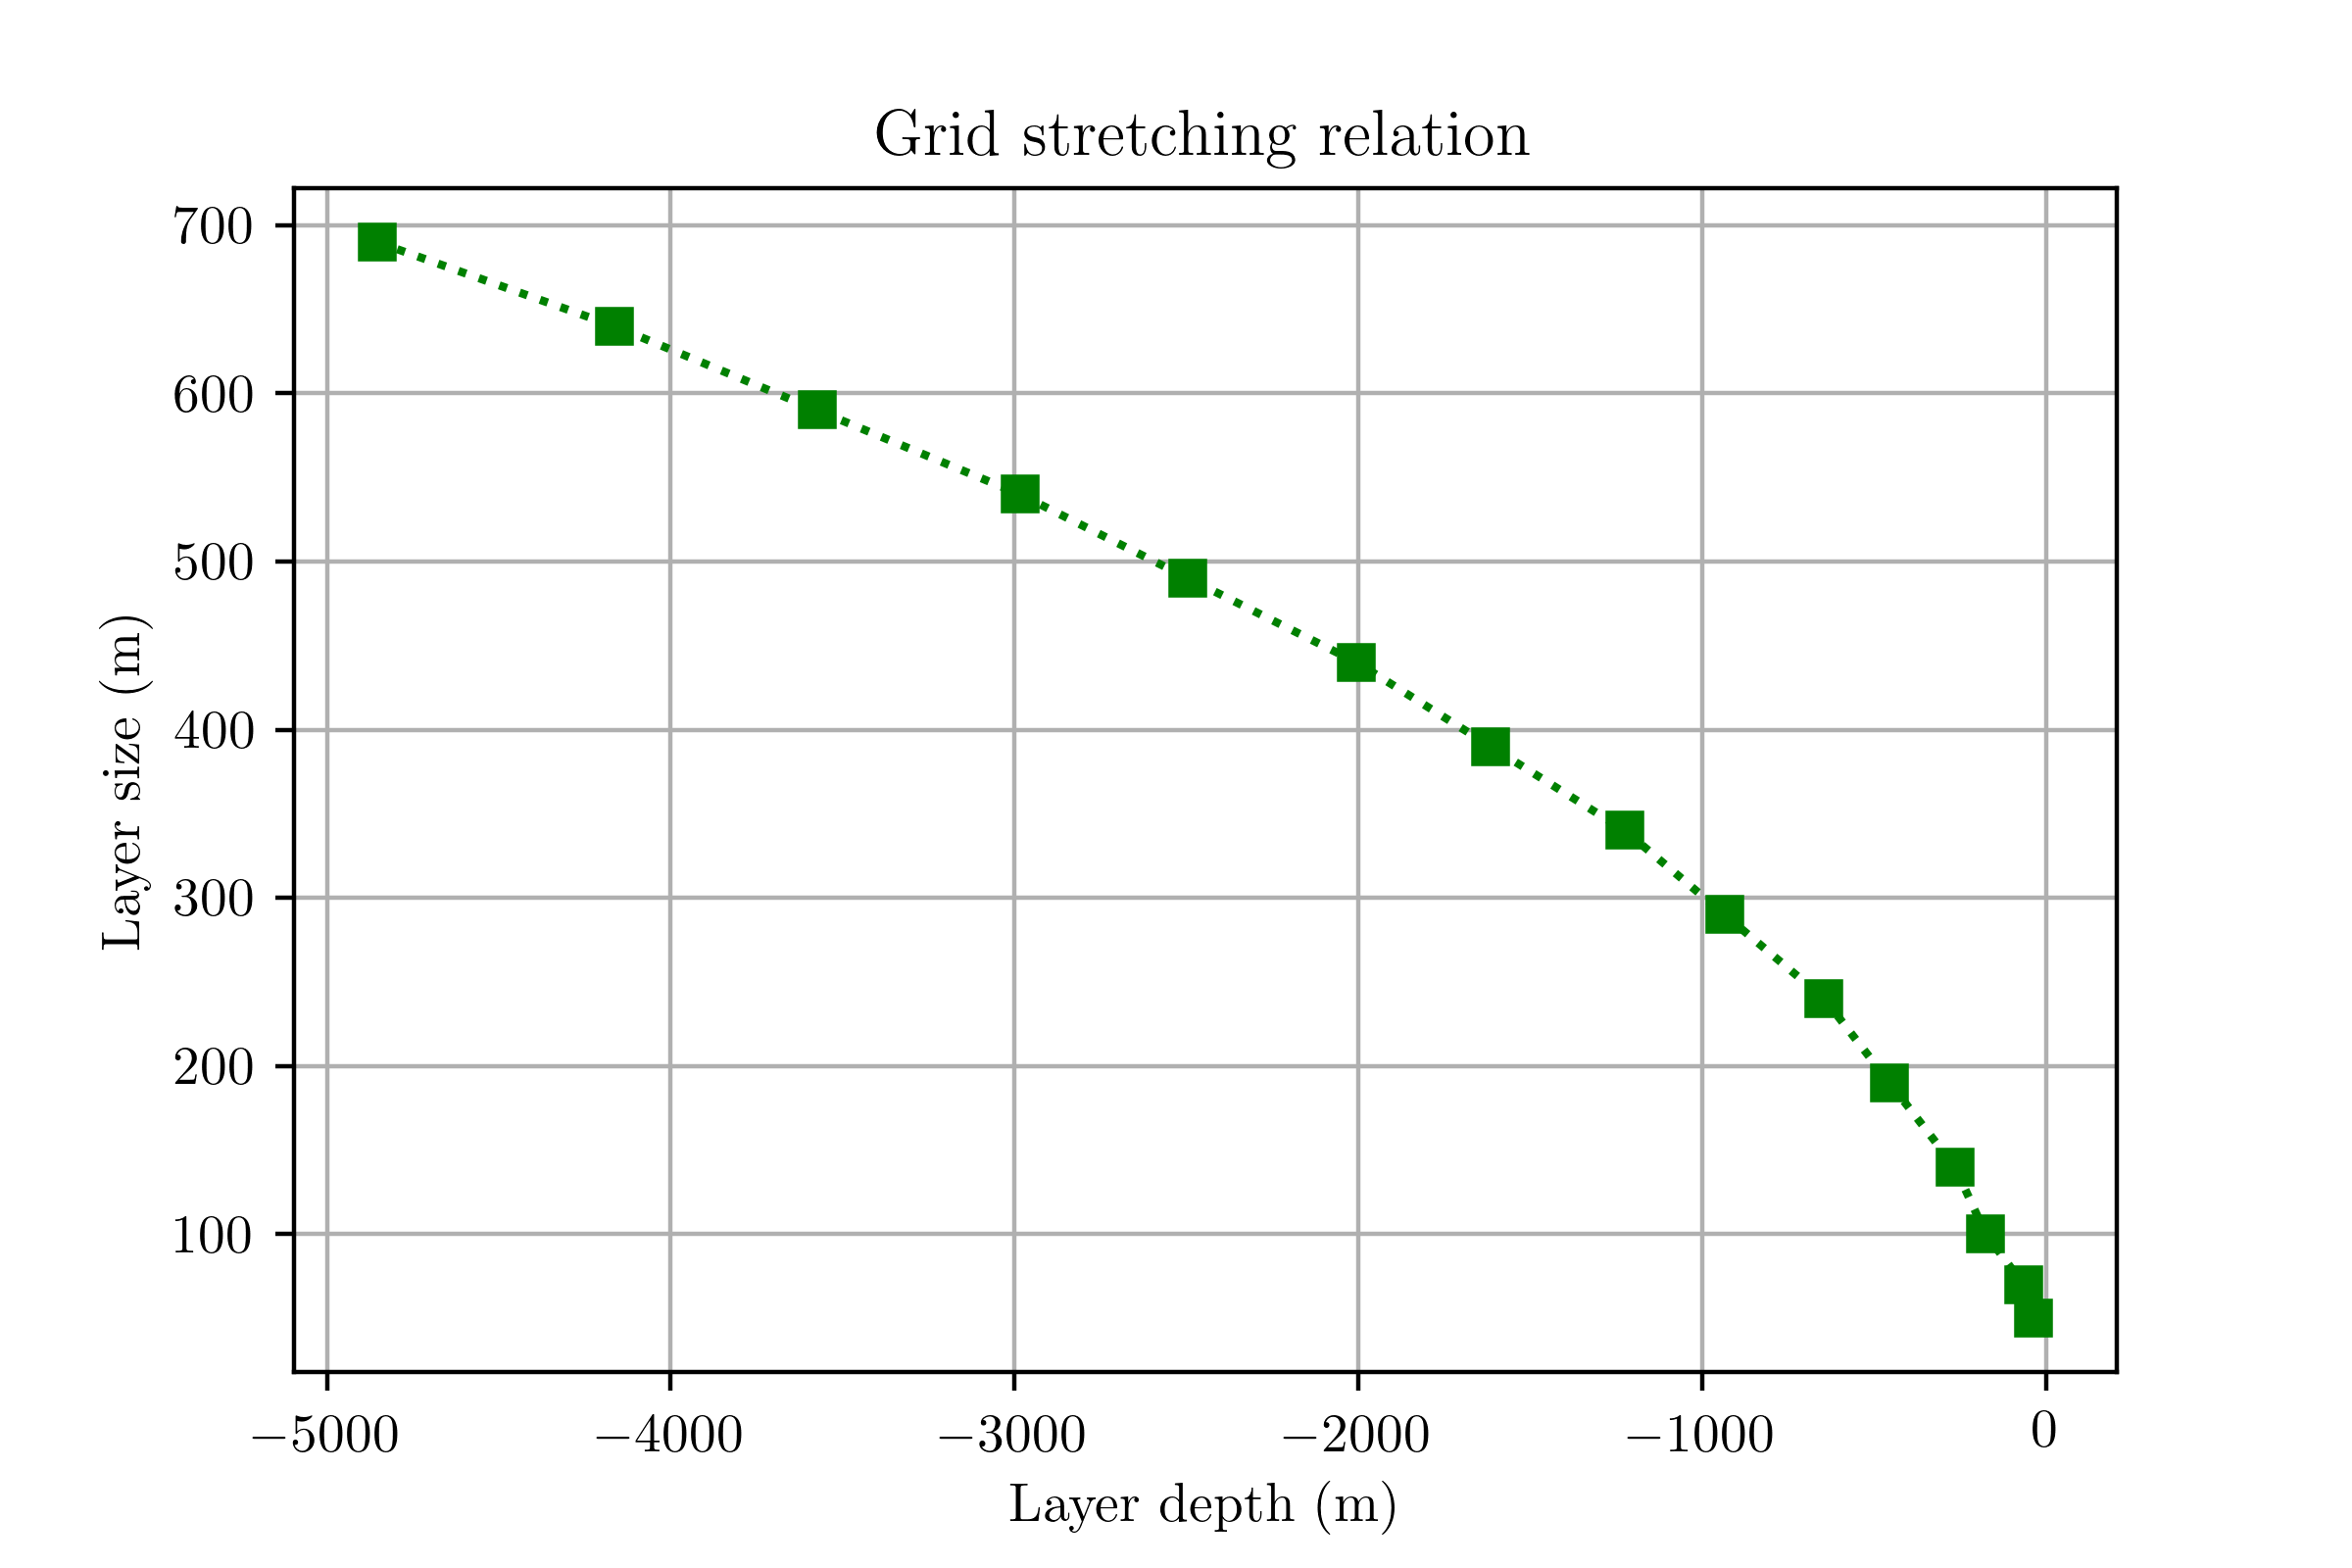
\includegraphics[width=\linewidth]{grid_stretching.png}
 	\caption{Grid stretching relation used}
 	\label{fig:gridstrech}
 \end{figure}

\subsubsection{Surface Forcings}
 Choosing the correct forcing for the ocean is very important. It is known that the MOC in general circulation models is highly sensitive too even small changes in surface forcings (\cite{Milliff1999May}). Attempts at making these forcings highly idealized have often been made in the past with varying rates of success. In this paper we will however use idealized forcings. Noting the fact, that this will probably induce the aforementioned errors in deep ocean circulations.
 
 There were several methods that are explored when it comes to creating these idealized forcings. In the \cite{Mulder2017Jul} paper an analytic forcing profile was used for wind flux, SST and SSS. This however fails to capture seasonal changes in each of the forcings due to the earths axial tilt. Something that can bring about a huge effect on the strength of the MOC. To combat this change a compromise is proposed. The SSS, SST and heat flux profiles are taken as zonal means for each month in the earths rotation. While the Zonal wind stress is set to the simple profile proposed by \cite{bryan1987parameter}. The analytic profile used in the paper is not specified specifically. but it can quite easily be deduced from the profile's plot. The choice of this analytic profile was made over a zonally averaged and equatorial averaged forcing $\mu(\tau_x)$. These were both tested on the present day configuration to see which of these forcings most accurately captures the present day MOC. In \fref{sec:MOCSTREAM} a comparison with the present day MOC and BSF is made. 
 
 \subsubsection{MOC stream function} \label{sec:MOCSTREAM}
 
 The global Meridional Overturning Circulation $\Psi_{MOC}$ is defined as the zonally integrated meridional volume transport of water in the worlds oceans. It can be written down as:
 
 $$
 \Psi_{MOC}(y,z) = \int_{z}^{0} \int_{-180^{\circ}}^{180^{\circ}} v(x,y,z') dx dz'
 $$
Where $v$ is the meridional component of the velocity.
$ \Psi_{MOC}$ is thus a stream function of the zonally integrated volume transport in the Earth's water basins. Plotting this stream function can give a lot of insight into the deep water transport associated with the thermohaline circulation. In this paper we hope to capture these deep water transport formations as a 

\subsubsection{Barotropic Stream Function}

The Barotropic stream function $\Psi_{b}$ is defined as the depth integrated volume transport in the Earth's water basin. It is a usefull tool to look at the shape and Gyres associated with the major ocean current systems. These Stream functions can be a useful tool to compare this simplified model to an existing $4^{\circ}$ model.

%TODO write something on the major ocean currents.